% THIS DOCUMENT IS TAILORED TO REQUIREMENTS FOR SCIENTIFIC COMPUTING.  IT SHOULDN'T
% BE USED FOR NON-SCIENTIFIC COMPUTING PROJECTS
\documentclass[12pt]{article}

\usepackage{amsmath, mathtools}
\usepackage{amsfonts}
\usepackage{amssymb}
\usepackage{graphicx}
\usepackage{colortbl}
\usepackage{xr}
\usepackage{hyperref}
\usepackage{longtable}
\usepackage{xfrac}
\usepackage{tabularx}
\usepackage{float}
\usepackage{siunitx}
\usepackage{booktabs}
\usepackage{caption}
\usepackage{pdflscape}
\usepackage{afterpage}

\usepackage[round]{natbib}

%\usepackage{refcheck}

\hypersetup{
    bookmarks=true,         % show bookmarks bar?
      colorlinks=true,       % false: boxed links; true: colored links
    linkcolor=red,          % color of internal links (change box color with linkbordercolor)
    citecolor=green,        % color of links to bibliography
    filecolor=magenta,      % color of file links
    urlcolor=cyan           % color of external links
}

%% Comments

\usepackage{color}

\newif\ifcomments\commentstrue %displays comments
%\newif\ifcomments\commentsfalse %so that comments do not display

\ifcomments
\newcommand{\authornote}[3]{\textcolor{#1}{[#3 ---#2]}}
\newcommand{\todo}[1]{\textcolor{red}{[TODO: #1]}}
\else
\newcommand{\authornote}[3]{}
\newcommand{\todo}[1]{}
\fi

\newcommand{\wss}[1]{\authornote{blue}{SS}{#1}} 
\newcommand{\plt}[1]{\authornote{magenta}{TPLT}{#1}} %For explanation of the template
\newcommand{\an}[1]{\authornote{cyan}{Author}{#1}}

%% Common Parts

\newcommand{\progname}{Helmholtz-Coil-Current-Calculator-CAS741} % PUT YOUR PROGRAM NAME HERE
\newcommand{\authname}{Reyhaneh Norouziani} % AUTHOR NAMES                  

\usepackage{hyperref}
    \hypersetup{colorlinks=true, linkcolor=blue, citecolor=blue, filecolor=blue,
                urlcolor=blue, unicode=false}
    \urlstyle{same}
                                


% For easy change of table widths
\newcommand{\colZwidth}{1.0\textwidth}
\newcommand{\colAwidth}{0.13\textwidth}
\newcommand{\colBwidth}{0.82\textwidth}
\newcommand{\colCwidth}{0.1\textwidth}
\newcommand{\colDwidth}{0.05\textwidth}
\newcommand{\colEwidth}{0.8\textwidth}
\newcommand{\colFwidth}{0.17\textwidth}
\newcommand{\colGwidth}{0.5\textwidth}
\newcommand{\colHwidth}{0.28\textwidth}

% Used so that cross-references have a meaningful prefix
\newcounter{defnum} %Definition Number
\newcommand{\dthedefnum}{GD\thedefnum}
\newcommand{\dref}[1]{GD\ref{#1}}
\newcounter{datadefnum} %Datadefinition Number
\newcommand{\ddthedatadefnum}{DD\thedatadefnum}
\newcommand{\ddref}[1]{DD\ref{#1}}
\newcounter{theorynum} %Theory Number
\newcommand{\tthetheorynum}{TM\thetheorynum}
\newcommand{\tref}[1]{TM\ref{#1}}
\newcounter{tablenum} %Table Number
\newcommand{\tbthetablenum}{TB\thetablenum}
\newcommand{\tbref}[1]{TB\ref{#1}}
\newcounter{assumpnum} %Assumption Number
\newcommand{\atheassumpnum}{A\theassumpnum}
\newcommand{\aref}[1]{A\ref{#1}}
\newcounter{goalnum} %Goal Number
\newcommand{\gthegoalnum}{GS\thegoalnum}
\newcommand{\gsref}[1]{GS\ref{#1}}
\newcounter{instnum} %Instance Number
\newcommand{\itheinstnum}{IM\theinstnum}
\newcommand{\iref}[1]{IM\ref{#1}}
\newcounter{reqnum} %Requirement Number
\newcommand{\rthereqnum}{R\thereqnum}
\newcommand{\rref}[1]{R\ref{#1}}
\newcounter{nfrnum} %NFR Number
\newcommand{\rthenfrnum}{NFR\thenfrnum}
\newcommand{\nfrref}[1]{NFR\ref{#1}}
\newcounter{lcnum} %Likely change number
\newcommand{\lthelcnum}{LC\thelcnum}
\newcommand{\lcref}[1]{LC\ref{#1}}

\usepackage{fullpage}

\newcommand{\deftheory}[9][Not Applicable]
{
\newpage
\noindent \rule{\textwidth}{0.5mm}

\paragraph{RefName: } \textbf{#2} \phantomsection 
\label{#2}

\paragraph{Label:} #3

\noindent \rule{\textwidth}{0.5mm}

\paragraph{Equation:}

#4

\paragraph{Description:}

#5

\paragraph{Notes:}

#6

\paragraph{Source:}

#7

\paragraph{Ref.\ By:}

#8

\paragraph{Preconditions for \hyperref[#2]{#2}:}
\label{#2_precond}

#9

\paragraph{Derivation for \hyperref[#2]{#2}:}
\label{#2_deriv}

#1

\noindent \rule{\textwidth}{0.5mm}

}

\begin{document}

\title{Software Requirements Specification for \progname: Three-axis Helmholtz Coil System Current Calculator and Target Magnetic Force or Magnetic Torque} 
\author{\authname}
\date{\today}
	
\maketitle

~\newpage

\pagenumbering{roman}

\tableofcontents

~\newpage

\section*{Revision History}

\begin{tabularx}{\textwidth}{p{3cm}p{2cm}X}
\toprule {\bf Date} & {\bf Version} & {\bf Notes}\\
\midrule
Date 1 & 1.0 & Notes\\
Date 2 & 1.1 & Notes\\
\bottomrule
\end{tabularx}

~\\

~\newpage

\section{Reference Material}

This section records information for easy reference.

\subsection{Table of Units}

Throughout this document SI (Syst\`{e}me International d'Unit\'{e}s) is employed
as the unit system.  In addition to the basic units, several derived units are
used as described below.  For each unit, the symbol is given followed by a
description of the unit and the SI name.
~\newline

\renewcommand{\arraystretch}{1.2}
%\begin{table}[ht]
  \noindent \begin{tabular}{l l l} 
    \toprule		
    \textbf{symbol} & \textbf{unit} & \textbf{SI}\\
    \midrule 
    \si{\metre} & length & metre\\
    \si{\ampere} & electric current & Ampere\\
    \si{\tesla} & magnetic field & Tesla\\
     \si{\newton} & force & newton\\
    \bottomrule
  \end{tabular}
  %	\caption{Provide a caption}
%\end{table}

\subsection{Table of Symbols}

The table that follows summarizes the symbols used in this document along with
their units.  The choice of symbols was made to be consistent with the heat
transfer literature and with existing documentation for solar water heating
systems.  The symbols are listed in alphabetical order.

\renewcommand{\arraystretch}{1.2}
%\noindent \begin{tabularx}{1.0\textwidth}{l l X}
\noindent \begin{longtable*}{l l p{12cm}} \toprule
\textbf{symbol} & \textbf{unit} & \textbf{description}\\
\midrule 
$B_x$ & \si[per-mode=symbol]{\tesla} & Magnetic field along the x-axis \\
$B_y$ & \si[per-mode=symbol]{\tesla} & Magnetic field along the y-axis \\
$B_z$ & \si[per-mode=symbol]{\tesla} & Magnetic field along the z-axis \\
$F$ & \si[per-mode=symbol]{\newton} & Magnetic force \\
$H$ & \si[per-mode=symbol]{\ampere\per\metre} & Total magnetic field strength \\
$I_x$ & \si[per-mode=symbol]{\ampere} & Electric current through the x-axis coils \\
$I_y$ & \si[per-mode=symbol]{\ampere} & Electric current through the y-axis coils \\
$I_z$ & \si[per-mode=symbol]{\ampere} & Electric current through the z-axis coils \\
$Imax_x$ & \si[per-mode=symbol]{\ampere} & Maximum acceptable electric current through the x-axis coils \\
$Imax_y$ & \si[per-mode=symbol]{\ampere} & Maximum acceptable electric current through the y-axis coils \\
$Imax_z$ & \si[per-mode=symbol]{\ampere} & Maximum acceptable electric current through the z-axis coils \\
$l_x$ & \si[per-mode=symbol]{\metre} & Distance between the coils along the x-axis \\
$l_y$ & \si[per-mode=symbol]{\metre} & Distance between the coils along the y-axis \\
$l_z$ & \si[per-mode=symbol]{\metre} & Distance between the coils along the z-axis \\
$N_x$ & & Number of turns in the x-axis coil \\
$N_y$ & & Number of turns in the y-axis coil \\
$N_z$ & & Number of turns in the z-axis coil \\
$R_x$ & \si[per-mode=symbol]{\metre} & Radius of the coils along the x-axis \\
$R_y$ & \si[per-mode=symbol]{\metre} & Radius of the coils along the y-axis \\
$R_z$ & \si[per-mode=symbol]{\metre} & Radius of the coils along the z-axis \\
$\mathbf{\tau}$ & \si[per-mode=symbol]{\si{\newton\meter}} & Magnetic torque \\
$x$ & \si[per-mode=symbol]{\metre} & Position along the x-axis from the midpoint \\
$y$ & \si[per-mode=symbol]{\metre} & Position along the y-axis from the midpoint \\
$z$ & \si[per-mode=symbol]{\metre} & Position along the z-axis from the midpoint \\

\bottomrule
\end{longtable*}


\subsection{Abbreviations and Acronyms}

\renewcommand{\arraystretch}{1.2}
\begin{tabular}{lp{15cm}} 
  \toprule		
  \textbf{symbol} & \textbf{description}\\
  \midrule 
  A & Assumption\\
  DD & Data Definition\\
  GD & General Definition\\
  GS & Goal Statement\\
  IM & Instance Model\\
  LC & Likely Change\\
  PS & Physical System Description\\
  R & Requirement\\
  SRS & Software Requirements Specification\\
  \progname{} & Three-axis Helmholtz Coil System Current Calculator and Target Magnetic Force or Magnetic Torque\\
  \bottomrule
\end{tabular}\\

\newpage

\pagenumbering{arabic}

\section{Introduction}
{
Helmholtz coils are utilized primarily for their ability to produce a nearly uniform magnetic field, a feature crucial in various scientific research and practical applications. The design consists of two identical electromagnetic coils placed symmetrically along a common axis and separated by a distance equal to their radius, having the same electric current in the same direction. It facilitates precise control over the magnetic field's strength by adjusting the electric current flowing through the coils. Alternatively, a Maxwell coil configuration is formed if currents flow in opposite directions, resulting in a uniform magnetic field gradient at the center. This precision is essential for applications that demand specific magnetic force and torque on a magnetic particle to induce desired effects on materials or biological tissues. Calculating the target magnetic field and magnetic torque based on the characteristics of a Helmholtz Coil system and magnetic particles significantly impact a wide range of scientific, medical, and industrial applications.
}

\subsection{Purpose of Document}
{
The primary objective of this Software Requirements Specification (SRS) document is to outline the software requirements for creating a Three-axis Helmholtz Coil System Current Calculator for Target Magnetic Force and Magnetic Torque application. This document endeavors to provide a thorough understanding of the system's architecture, focusing on the project's objectives, operational principles, and essential definitions without focusing on the implementation specifics. It aims to establish a clear overview to facilitate software development, detailing the system's context, constraints, and the problem the project intends to solve. Furthermore, the document considers possible future enhancements and modifications, ensuring the system's adaptability and scalability to meet evolving requirements.
}

\subsection{Scope of Requirements} 
{
The project's scope is concentrated on developing a current calculator for a Three-axis Helmholtz Coil System that precisely determines the currents required to achieve a target magnetic force and torque at the system's central point. This calculator assumes an idealized scenario where the coil system is entirely isolated from any external magnetic fields, ensuring that calculations are unaffected by outside magnetic interference. The software's focus is on theoretical predictions and is not concerned with the physical implementation or the dynamic adaptation to environmental changes. The resulting tool will be critical for applications necessitating precise magnetic field manipulation, serving as a foundational resource for further experimental and practical exploration.
}  

\subsection{Characteristics of Intended Reader} \label{sec_IntendedReader}
{
The reader should have a strong foundation in physics, particularly in electromagnetism. A university-level understanding, at least at the undergraduate level, is expected. Familiarity with differential calculus and vector analysis is necessary since the project involves calculating magnetic field gradients and currents.

}

\subsection{Organization of Document}
{
The document is organized into several key sections to present the software requirements specification systematically. After the introduction, which outlines the document's purpose, scope, and definitions, the general system description provides an overview of the system's context and interactions. Subsequently, The system description discusses the problem, assumptions, and dependencies. The requirements section details the functional and nonfunctional requirements, followed by a discussion on likely and unlikely changes to the system. The document also includes traceability matrices to illustrate the relationships between different components of the SRS, ensuring clear reference and maintenance.
}

\section{General System Description}

This section provides general information about the system.  It identifies the
interfaces between the system and its environment, describes the user
characteristics and lists the system constraints.
\subsection{System Context}

{
The Figure \ref{Fig_SystemContext} illustrates the user and software interaction. Users input the specifications of a three-axis Helmholtz Coil system, along with the desired magnetic force, torque, and the magnetic moment of the targeted particle. The software processes these inputs to calculate the precise current needed for each coil to achieve the specified magnetic torque and magnetic force. Then, it outputs this information back to the user.
}

\begin{figure}[H]
\begin{center}
 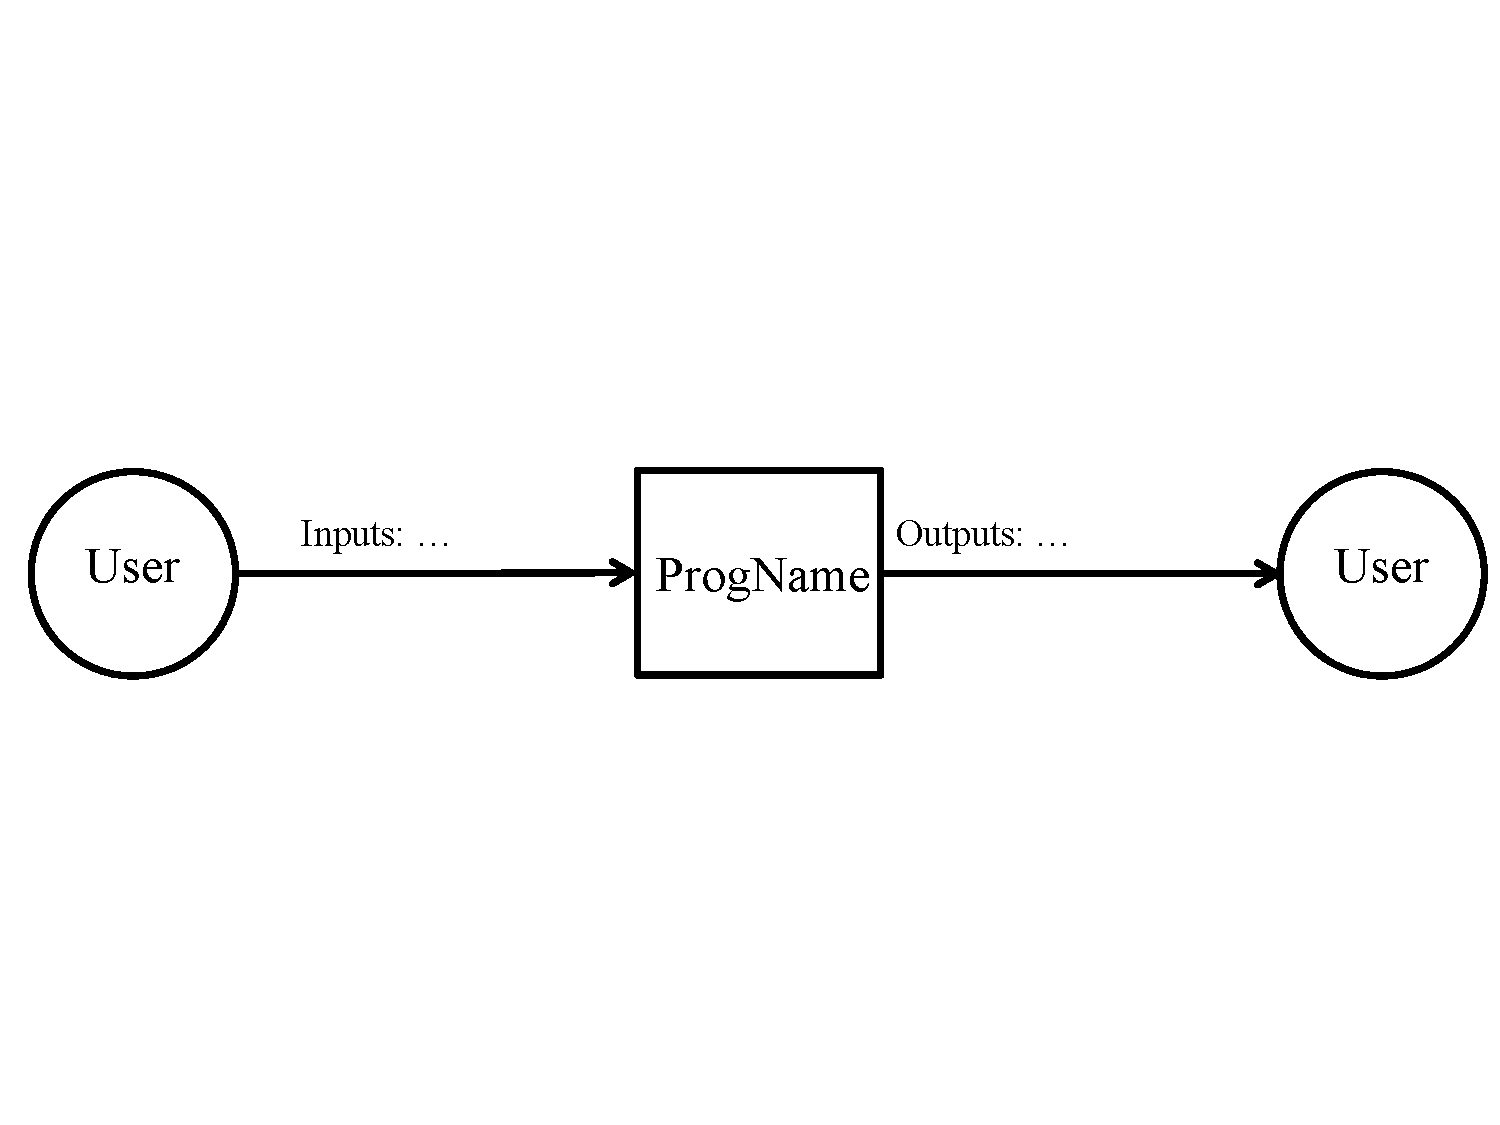
\includegraphics[width=1.0\textwidth]{SystemContextFigure}
\caption{System Context}
\label{Fig_SystemContext} 
\end{center}
\end{figure}

\begin{itemize}
\item User Responsibilities:
\begin{itemize}
\item Provide accurate and precise input data, such as the characteristics of the Helmholtz coil system, target force, target torque, and magnetic moment.

\end{itemize}
\item \progname{} Responsibilities:
\begin{itemize}
\item Accurately calculate the current required in each coil based on the user-provided input data.
\item Present the calculated data in a clear and understandable format to the user.
\item Verify that the calculated current is within the operational range of the system, ensuring the values are practical and safe for real-world application.
\end{itemize}
\end{itemize}
{
The Helmholz-Coil-Current-Calculator-CAS741 software is primarily utilized by researchers and scientists engaged in designing and working with Helmholtz coil systems. These professionals rely on the software to accurately generate specific magnetic forces and torques for experimental and investigative purposes in laboratory settings. While the software plays a crucial role in the research and development phase, it is not typically classified as mission-critical or safety-critical; however, it does demand high precision and reliability to ensure the validity of scientific experiments and the integrity of data collected.
}

\subsection{User Characteristics} \label{SecUserCharacteristics}

The users of this program are typically researchers and scientists with a solid foundation in physics, particularly in electromagnetism. They are expected to have experience with magnetic coil systems and a good grasp of mathematical concepts required to understand and utilize the software's calculations. Their expertise allows them to interpret the software's output accurately and integrate it into their scientific work, applying the calculated forces and torques to their specific applications in research and experimental setups.

\subsection{System Constraints}

There is no system constraint for this program.

\section{Specific System Description}

This section presents the problem at a high-level concept, followed by the solution characteristics specification which includes assumptions, theories, definitions, and instance models.

\subsection{Problem Description} \label{Sec_pd}

The problem description for the Helmholz-Coil-Current-Calculator-CAS741 project addresses the challenge of calculating the precise currents needed for a three-axis Helmholtz coil system to generate specific magnetic forces and torques. This complex task requires integrating electromagnetic theory and applying mathematical models to control the magnetic field within the coil setup. The solution must be precise, reliable, and user-friendly to support scientific research and experimentation where accurate magnetic field manipulation is critical.
\subsubsection{Terminology and  Definitions}
This subsection provides a list of terms used in the subsequent
sections and their meaning, with the purpose of reducing ambiguity and making it easier to correctly understand the requirements:


\begin{itemize}

\item Magnetic Field: A magnetic field is a vector field produced by a current flow or a magnetized material

\item Magnetic Moment: The magnetic moment is a vector quantity that represents the magnetic strength and orientation of a magnet or other object that produces a magnetic field. It's a fundamental property of magnetic materials and is typically caused by the orbital and spin motions of electrons within atoms.

\item Coil: A coil, in the context of a Helmholtz coil, it specifically refers to a configuration of wire loops designed to create a uniform magnetic field within the volume of the coil.
\item Magnetic torque: The Magnetic torque is a measure of the turning force on an object caused by the magnetic field and the magnetic moment of the object. It determines how strongly an object (which has a magnetic moment) will align with the magnetic field.
\item Magnetic force: The Magnetic force refers to the force exerted by a magnetic field on a moving charge, a current-carrying wire, or a material with a magnetic moment.
\end{itemize}

\subsubsection{Physical System Description} \label{sec_phySystDescrip}

The physical system of Three-axis Helmholtz Coil System, as shown in Figure \ref{helmholtz},
includes the following elements:

\begin{itemize}

\item[PS1:]  two coils along the x-axis

\item[PS2:]  two coils along the y-axis

\item[PS3:]  two coils along the z-axis


\end{itemize}

 \begin{figure}[h!]
 \begin{center}
 %\rotatebox{-90}
 {
  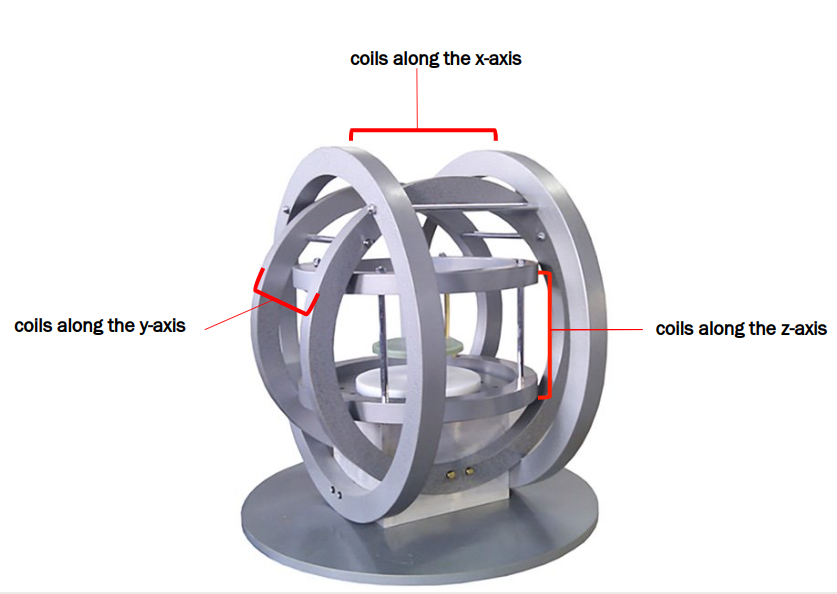
\includegraphics[width=0.5\textwidth]{hcs.png}
 }
 \caption{\label{helmholtz} Three-axis Helmholtz Coil System}
 \end{center}
 \end{figure}

\subsubsection{Goal Statements}

Given the parameters of a Three-axis Helmholtz coil system, which include the number of turns on each coil, the radius of each coil, the distance between the coils, the maximum current each coil has access to, and the desired magnetic field strength the goal statement is:

\begin{itemize}

\item[GS\refstepcounter{goalnum}\thegoalnum \label{G_force}:] Calculate the current required for each coil to achieve the target magnetic force at the center
\item[GS\refstepcounter{goalnum}\thegoalnum \label{G_torque}:] Calculate the current required for each coil to achieve the target magnetic torque at the center

\end{itemize}

\subsection{Solution Characteristics Specification}


The instance models that govern \progname{} are presented in
Subsection~\ref{sec_instance}.  The information to understand the meaning of the
instance models and their derivation is also presented, so that the instance
models can be verified.

\subsubsection{Assumptions} \label{sec_assumpt}
This section simplifies the original problem and helps in developing the
theoretical model by filling in the missing information for the physical system.
The numbers given in the square brackets refer to the theoretical model [TM],
general definition [GD], data definition [DD], instance model [IM], or likely
change [LC], in which the respective assumption is used.

\begin{itemize}

\item[A\refstepcounter{assumpnum}\theassumpnum \label{A_directPower}:]
The system is assumed to be powered by a direct current source, ensuring that the generated magnetic field is steady.

\item[A\refstepcounter{assumpnum}\theassumpnum \label{A_noExtField}:]
It is assumed there are no significant external magnetic fields present that could interfere with the magnetic field generated by the Helmholtz coil system. This ensures that the magnetic field within the operational area is solely due to the coils themselves.

\item[A\refstepcounter{assumpnum}\theassumpnum \label{A_generateWithinCenter}:]
We assume that the target magnetic force and torque is to be generated within the center of the Helmholtz coil.

\end{itemize}

\subsubsection{Theoretical Models}\label{sec_theoretical}
This section focuses on the general equations and laws that \progname{} is based
on.  

~\newline
\noindent
\deftheory
% #2 refname of theory
{TM:FBD}
% #3 label
{Force on a magnetic dipole}
% #4 equation
{
\begin{equation}
\vec{F} = (\vec{m} \cdot \nabla) \vec{B}
\end{equation}
}
% #5 description
{
The equation represents the force on a magnetic dipole in an inhomogeneous magnetic field. Here, \( \mathbf{F} \)(\si{\newton}) is the force, \( \mathbf{m} \)(\si{\ampere\square\meter}) is the magnetic moment,\( \mathbf{B} \)(\si{\tesla}) is the magnetic field. }
% #6 Notes
{
None.
}
% #7 Source
{
  \url{}
}
% #8 Referenced by
{
\iref{cnf}
}
% #9 Preconditions
{
None
}
% #1 derivation - not applicable by default
{}
~\newline
\noindent
\deftheory
% #2 refname of theory
{TM:TBD}
% #3 label
{Torque on a magnetic dipole}
% #4 equation
{
\begin{equation}
\vec{\tau} = \vec{m} \times \vec{B}
\end{equation}
}
% #5 description
{
The equation represents magnetic torque \( \mathbf{\tau} \) (\si{\newton\meter}) experienced by a magnetic dipole in a uniform magnetic field. There the torque \( \mathbf{\tau} \) (\si{\newton\meter})is given by the vector cross product of the magnetic moment \( \mathbf{m} \)(\si{\ampere\square\meter}) and the magnetic field \( \mathbf{B} \)(\si{\tesla}).
}
% #6 Notes
{
None.
}
% #7 Source
{
  \url{}
}
% #8 Referenced by
{
	\iref{cnt}
}
% #9 Preconditions
{
None
}
% #1 derivation - not applicable by default
{}
~\newline
\noindent
\deftheory
% #2 refname of theory
{TM:BSL}
% #3 label
{Biot-Savart law}
% #4 equation
{
\begin{equation}
\vec{B} = \frac{\mu_0}{4\pi} \frac{Id\vec{l} \times \vec{r}}{r^2}
\end{equation}
}
% #5 description
{
The equation gives the magnetic flux density $\vec{B}$ (\si{\tesla}) generated by a constant electric current $I$ (\si{\ampere}) of a current-carrying wire at position $r$ (\si{\meter}) in 3D space where $\mu_0$ is the magnetic constant (\si{\newton\per\ampere\squared})and $\vec{r}$ is the position vector from the current element to the point where the field is being calculated.}
% #6 Notes
{
None.
}
% #7 Source
{
  \url{}
}
% #8 Referenced by
{
  \dref{mfc}
}
% #9 Preconditions
{
None
}
% #1 derivation - not applicable by default
{
}

~\newline

\subsubsection{General Definitions}\label{sec_gendef}

This section collects the laws and equations that will be used in building the
instance models.

~\newline

\noindent
\begin{minipage}{\textwidth}
\renewcommand*{\arraystretch}{1.5}
\begin{tabular}{| p{\colAwidth} | p{\colBwidth}|}
\hline
\rowcolor[gray]{0.9}
Number& GD\refstepcounter{defnum}\thedefnum \label{mfc}\\
\hline
Label &\bf Magnetic field along the axis of a coil \\
\hline
% Units&$MLt^{-3}T^0$\\
% \hline
SI Units&(\si{\tesla})\\
\hline
Equation&${B} = \frac{ {N} \mu_0 IR}{2(x^2 + R^2)^{3/2}}$  \\
\hline
Description &
The equation represents the magnetic field $B$ along the axis of a coil with multiple turns.

\begin{itemize}
    \item \(B\): The magnetic field at a point along the axis of the coil(\si{\tesla}).
    \item \(N\): The number of turns in the coil. Each turn contributes to the total magnetic field, so the field strength is proportional to the number of turns.
    \item \(\mu_0\): The magnetic constant or the permeability of free space, which is \(4\pi \times 10^{-7}\, \si{\tesla\meter\per\ampere}\) (\si{\tesla\meter\per\ampere}).
    \item \(I\): The current through the coil(\si{\ampere}).
    \item \(R\): The radius of the coil(\si{\meter}).
    \item \(x\): The distance from the center of the coil along its axis to the point(\si{\meter}).
\end{itemize}
\\
\hline
  Source &  \\
  \hline
  Ref.\ By & \dref{cfmh}, \dref{mfcm}\\
  \hline
\end{tabular}
\end{minipage}\\

\subsubsection*{Detailed derivation of magnetic field along the axis of it }
{For a small current element \(Id\mathbf{l}\) on the loop, the \tref{TM:BSL} gives the magnetic field contribution \(d\mathbf{B}\) at point \(x\) on the axis.\\

By symmetry, only the component of \(d\mathbf{B}\) that is along the axis (the \(x\)-component) contributes to the net field at point \(x\). The field due to each element is directed according to the right-hand rule, which, given your description, points to the right along the axis of the loop for the entire loop.\\


Using the Biot-Savart Law, the \(x\)-component of the field due to the element is \(dB_x = dB \cdot \sin(\theta)\), where \(\theta\) is the angle between \(d\mathbf{l}\) and \(\mathbf{r}\). Because \(\sin(\theta) = \frac{r}{R}\) and \(r = \sqrt{x^2 + R^2}\), the \(x\)-component of \(d\mathbf{B}\) is given by:
\[
dB_x = \frac{\mu_0}{4\pi} \frac{IdlR}{(x^2 + R^2)^{3/2}}
\]
\\
The integral \(\int d\mathbf{l}\) around the loop gives the circumference \(2\pi R\), so the net magnetic field at point \(x\) is:
\[
B_x = \frac{\mu_0}{4\pi} \frac{I}{(x^2 + R^2)^{3/2}} \int d\mathbf{l} = \frac{\mu_0 IR}{2(x^2 + R^2)^{3/2}}
\]Which is the magnetic field at a distance \(x\) from the center of the loop along its axis. \\


For a coil with \( N \) turns, this expression is multiplied by \( N \), since each turn contributes to the magnetic field at the point \( x \). Therefore, the total magnetic field \( B_x \) due to a coil with \( N \) turns is
\[
B_x = \frac{N \mu_0 I R^2}{2(x^2 + R^2)^{3/2}}
\]

These calculations can be generalized for the y and z axis, allowing for a comprehensive analysis of the magnetic field in three-dimensional space.
}

\noindent
\begin{minipage}{\textwidth}
\renewcommand*{\arraystretch}{1.5}
\begin{tabular}{| p{\colAwidth} | p{\colBwidth}|}
\hline
\rowcolor[gray]{0.9}
Number& GD\refstepcounter{defnum}\thedefnum \label{cfmh}\\
\hline
Label &\bf Magnetic field in the center of a Helmholtz Coil along the axis of it \\
\hline
% Units&$MLt^{-3}T^0$\\
% \hline
SI Units&(\si{\tesla})\\
\hline
Equation&$B= \frac{\mu_0 N I R^2}{2(x^2 + R^2)^{\frac{3}{2}}} + \frac{\mu_0 N I R^2}{2((l - x)^2 + R^2)^{\frac{3}{2}}} $ \\
\hline
Description &
In a Helmholtz coil setup, we have two identical circular coils that are spaced a distance apart. Each coil produces its own magnetic field \dref{mfc}, and because the coils are arranged along the same axis and the currents flow in the same direction, the magnetic fields generated by the individual coils add up constructively in the space between them.

\begin{itemize}
    \item \(B\): The magnetic field at a point along the axis of the coil(\si{\tesla}).
    \item \(N\): The number of turns in the coil. Each turn contributes to the total magnetic field, so the field strength is proportional to the number of turns.
    \item \(\mu_0\): The magnetic constant or the permeability of free space, which is \(4\pi \times 10^{-7}\, \si{\tesla\meter\per\ampere}\) (\si{\tesla\meter\per\ampere}).
    \item \(I\): The current through the coil(\si{\ampere}).
    \item \(R\): The radius of the coil(\si{\meter}).
    \item \(x\): The distance from the center of the coil along its axis to the point(\si{\meter}).
    \item \(l\): The distance between two coils(\si{\meter}).
\end{itemize}
\\
\hline
  Source &  \\
  \hline
  Ref.\ By & \iref{cnt}\\
  \hline
\end{tabular}
\end{minipage}\\

\subsubsection*{Detailed derivation of magnetic field in the center of a Helmholtz Coil along the axis of it  }
In a Helmholtz coil setup, we have two identical circular coils that are spaced a distance apart equal to their radius. Each coil produces its own magnetic field \dref{mfc}, and because the coils are arranged along the same axis and the currents flow in the same direction, the magnetic fields generated by the individual coils add up constructively in the space between them.


\noindent
\begin{minipage}{\textwidth}
\renewcommand*{\arraystretch}{1.5}
\begin{tabular}{| p{\colAwidth} | p{\colBwidth}|}
\hline
\rowcolor[gray]{0.9}
Number& GD\refstepcounter{defnum}\thedefnum \label{mfcm}\\
\hline
Label &\bf Magnetic field in the center of a maxwell Coil along the axis of it \\
\hline
% Units&$MLt^{-3}T^0$\\
% \hline
SI Units&(\si{\tesla})\\
\hline
Equation&$B= \frac{\mu_0 N I R^2}{2(x^2 + R^2)^{\frac{3}{2}}} - \frac{\mu_0 N I R^2}{2((l - x)^2 + R^2)^{\frac{3}{2}}} $ \\
\hline
Description &
In a Helmholtz coil setup, we have two identical circular coils that are spaced a distance apart. Each coil produces its own magnetic field, and because the coils are arranged along the same axis and the currents flow in the same direction, the magnetic fields generated by the individual coils add up constructively in the space between them.

\begin{itemize}
    \item \(B\): The magnetic field at a point along the axis of the coil(\si{\tesla}).
    \item \(N\): The number of turns in the coil. Each turn contributes to the total magnetic field, so the field strength is proportional to the number of turns.
    \item \(\mu_0\): The magnetic constant or the permeability of free space, which is \(4\pi \times 10^{-7}\, \si{\tesla\meter\per\ampere}\) (\si{\tesla\meter\per\ampere}).
    \item \(I\): The current through the coil(\si{\ampere}).
    \item \(R\): The radius of the coil(\si{\meter}).
    \item \(x\): The distance from the center of the coil along its axis to the point(\si{\meter}).
    \item \(l\): The distance between two coils(\si{\meter}).
\end{itemize}
\\
\hline
  Source &  \\
  \hline
  Ref.\ By & \iref{cnf}\\
  \hline
\end{tabular}
\end{minipage}\\

\subsubsection*{Detailed derivation of magnetic field along the axis of a coil }
In a Maxwell coil setup, we have two identical circular coils that are spaced a distance apart equal to their radius. Each coil produces its own magnetic field, and because the coils are arranged along the same axis and the currents flow in the opposite direction, the magnetic fields generated by the individual coils are oppose each other.

\subsubsection{Data Definitions}\label{sec_datadef}

This section collects and defines all the data needed to build the instance
models. The dimension of each quantity is also given. 
~\newline

\subsubsection{Instance Models} \label{sec_instance}    

This section transforms the problem defined in Section~\ref{Sec_pd} into 
one which is expressed in mathematical terms. It uses concrete symbols defined 
in Section~\ref{sec_datadef} to replace the abstract symbols in the models 
identified in Sections~\ref{sec_theoretical} and~\ref{sec_gendef}.

The goals \gsref{G_force} and \gsref{G_torque} are solved by \iref{cnf} and \iref{cnt} respectively.

~\newline

%Instance Model 1

\noindent
\begin{minipage}{\textwidth}
\renewcommand*{\arraystretch}{1.5}
\begin{tabular}{| p{\colAwidth} | p{\colBwidth}|}
  \hline
  \rowcolor[gray]{0.9}
  Number& IM\refstepcounter{instnum}\theinstnum \label{cnf}\\
  \hline
  Label& \bf Current needed for target force\\
  \hline
  Input& $\vec{f}$, $\vec{m}$, $R_x$, $R_y$, $R_z$, $l_x$, $l_y$, $l_z$, $N_x$, $N_y$, $N_z$,$\text{max\_}I_x$, $\text{max\_}I_y$, $\text{max\_}I_z$ \\
 
  \hline
  Output& $\vec{I_1} =[-\frac{2\left( \frac{l_{x}^{2}}{4}+R_{x}^{2} \right) ^{5/2}}{3\mu _0N_xR_{x}^{2}l_xm_x}F_x, -\frac{2\left( \frac{l_{y}^{2}}{4}+R_{y}^{2} \right) ^{5/2}}{3\mu _0N_yR_{y}^{2}l_ym_y}F_y,-\frac{2\left( \frac{l_{z}^{2}}{4}+R_{z}^{2} \right) ^{5/2}}{3\mu _0N_zR_{z}^{2}l_zm_z}F_z]$\\
  \hline
  Description& With condisitons\aref{A_generateWithinCenter},\aref{A_noExtField},and $B$ from \dref{mfcm} we calculate the spatial derivative of $B_x$ with respect to x, which describes how the field changes along the axis. 

$\frac{d}{dx}B_x\left( x \right) =-\frac{3\mu _0N_xI_xR_{x}^{2}x}{2\left( x^2+R_{x}^{2} \right) ^{5/2}}+\frac{3\mu _0N_xI_xR_{x}^{2}\left( x-l_x \right)}{2\left( \left( l_x-x \right) ^2+R_{x}^{2} \right) ^{5/2}}$

The gradient is then evaluated at the midpoint between the two coils $x=l/2$, which is typically where measurements are taken

$\left. \frac{d}{dx}B_x\left( x \right) \right|_{x=\frac{l_x}{2}}=-\frac{3\mu _0N_xI_xR_{x}^{2}l_x}{2\left( \frac{l_{x}^{2}}{4}+R_{x}^{2} \right) ^{5/2}}$

By using \dref{TM:FBD} we reach to the equation below.

$F_x=-\frac{3\mu _0N_xI_xR_{x}^{2}l_x}{2\left( \frac{l_{x}^{2}}{4}+R_{x}^{2} \right) ^{5/2}}m_x$

The following relationship is derived by rearranging the previous equation to isolate the current, allowing for the calculation of the current needed to achieve a specific magnetic force.

$\Longrightarrow I_x=-\frac{2\left( \frac{l_{x}^{2}}{4}+R_{x}^{2} \right) ^{5/2}}{3\mu _0N_xR_{x}^{2}l_xm_x}F_x$

The same calculation can be applied for $I_y$ and $I_z$

$\Longrightarrow I_y=-\frac{2\left( \frac{l_{y}^{2}}{4}+R_{y}^{2} \right) ^{5/2}}{3\mu _0N_yR_{y}^{2}l_ym_y}F_y$

$\Longrightarrow I_z=-\frac{2\left( \frac{l_{z}^{2}}{4}+R_{z}^{2} \right) ^{5/2}}{3\mu _0N_zR_{z}^{2}l_zm_z}F_z$

  \\
  \hline
  Sources& \\
  \hline
  Ref.\ By & \rref{R_Calculate1}\\
  \hline
\end{tabular}
\end{minipage}\\
%~\newline

%Instance Model 2

\noindent
\begin{minipage}{\textwidth}
\renewcommand*{\arraystretch}{1.5}
\begin{tabular}{| p{\colAwidth} | p{\colBwidth}|}
  \hline
  \rowcolor[gray]{0.9}
  Number& IM\refstepcounter{instnum}\theinstnum \label{cnt}\\
  \hline
  Label& \bf Current needed for target torque\\
  \hline
  Input& $\vec{\tau}$, $\vec{m}$, $R_x$, $R_y$, $R_z$, $l_x$, $l_y$, $l_z$, $N_x$, $N_y$, $N_z$,$\text{max\_}I_x$, $\text{max\_}I_y$, $\text{max\_}I_z$ \\

  \hline
  Output& $\vec{I_2}=\left[\frac{1}{\frac{m^2\mu _0N_xR_{x}^{2}}{\left( \frac{l_{x}^{2}}{4}+R_{x}^{2} \right) ^{3/2}}}\left[ \tau _ym_z-\tau _zm_y \right] ,\frac{1}{\frac{m^2\mu _0N_yR_{y}^{2}}{\left( \frac{l_{y}^{2}}{4}+R_{y}^{2} \right) ^{3/2}}}\left[ \tau _zm_x-\tau _xm_z \right], \frac{1}{\frac{m^2\mu _0N_zR_{z}^{2}}{\left( \frac{l_{z}^{2}}{4}+R_{z}^{2} \right) ^{3/2}}}\left[ \tau _xm_y-\tau _ym_x \right]\right]$\\
  \hline
    Description& With condisitons\aref{A_generateWithinCenter},\aref{A_noExtField},and $B$ from \dref{cfmh} we calculate the spatial derivative of $B_x$ with respect to x, which describes how the field changes along the axis. 

  \\
  \hline
  Sources&  \\
  \hline
  Ref.\ By & \rref{R_Calculate2}\\
  \hline
\end{tabular}
\end{minipage}\\
%~\newline

\subsubsection*{Derivation of Current needed for target torque}

Initially, expressions for $B$ specifically at $B_x\left( \frac{l_x}{2} \right)$ from $B$ from \dref{cfmh} are provided.

$B_x\left( x \right) =\frac{\mu _0N_xI_xR_{x}^{2}}{2\left( x^2+R_{x}^{2} \right) ^{3/2}}+\frac{\mu _0N_xI_xR_{x}^{2}}{2\left( \left( l_x-x \right) ^2+R_{x}^{2} \right) ^{3/2}}$

$B_x\left( \frac{l_x}{2} \right) =\frac{\mu _0N_xI_xR_{x}^{2}}{\left( \frac{l_{x}^{2}}{4}+R_{x}^{2} \right) ^{3/2}}=C_xI_x$

The overall magnetic field is decomposed into components parallel ($\vec{B}_{\parallel}$) and perpendicular ( $\vec{B}_{\bot}$ to the magnetic moment, noting that only the perpendicular component contributes to the torque. 

$\vec{B}=\vec{B}_{\bot}+\vec{B}_{\parallel}$

$\vec{m}\cdot \vec{B}_{\bot}=0$

$\vec{m}\times \vec{B}_{\parallel}=0$

$\vec{\tau}\begin{array}{l}
 =\vec{m}\times \vec{B}\\
 =\vec{m}\times \left( \vec{B}_{\bot}+\vec{B}_{\parallel} \right)\\
 =\vec{m}\times \vec{B}_{\bot}+\underset{=0}{\underbrace{\vec{m}\times \vec{B}_{\parallel}}}\\
 =\vec{m}\times \vec{B}_{\bot}\\
\end{array}$

By using \tref{TM:TBD}:

$\vec{\tau}\times \vec{m}=\left( \vec{m}\times \vec{B}_{\bot} \right) \times \vec{m}$

$\vec{\tau}\times \vec{m}=m^2\vec{B}_{\bot}$

$\Rightarrow \vec{B}_{\bot}=\frac{1}{m^2}\vec{\tau}\times \vec{m}$

$\vec{B}_{\parallel}=0$

$\Rightarrow \vec{B}=\frac{1}{m^2}\vec{\tau}\times \vec{m}$

$B_x=\frac{1}{m^2}\left[ \tau _ym_z-\tau _zm_y \right] $

$\Rightarrow I_x=\frac{1}{\frac{m^2\mu _0N_xR_{x}^{2}}{\left( \frac{l_{x}^{2}}{4}+R_{x}^{2} \right) ^{3/2}}}\left[ \tau _ym_z-\tau _zm_y \right] $

$\Rightarrow I_y=\frac{1}{\frac{m^2\mu _0N_yR_{y}^{2}}{\left( \frac{l_{y}^{2}}{4}+R_{y}^{2} \right) ^{3/2}}}\left[ \tau _zm_x-\tau _xm_z \right] $

$\Rightarrow I_z=\frac{1}{\frac{m^2\mu _0N_zR_{z}^{2}}{\left( \frac{l_{z}^{2}}{4}+R_{z}^{2} \right) ^{3/2}}}\left[ \tau _xm_y-\tau _ym_x \right] $


\subsubsection{Input Data Constraints} \label{sec_DataConstraints}    

Table~\ref{TblInputVar} shows the data constraints on the input output
variables.  The column for physical constraints gives the physical limitations
on the range of values that can be taken by the variable.  The column for
software constraints restricts the range of inputs to reasonable values.  The
software constraints will be helpful in the design stage for picking suitable
algorithms.  The constraints are conservative, to give the user of the model the
flexibility to experiment with unusual situations.  The column of typical values
is intended to provide a feel for a common scenario.  The uncertainty column
provides an estimate of the confidence with which the physical quantities can be
measured.  This information would be part of the input if one were performing an
uncertainty quantification exercise.


\begin{table}[H]
  \caption{Input Variables} \label{TblInputVar}
  \renewcommand{\arraystretch}{1.2}
\noindent \begin{longtable*}{l l l l c} 
  \toprule
  \textbf{Var} & \textbf{Physical Constraints} & \textbf{Software Constraints} &
                             \textbf{Typical Value} & \textbf{Uncertainty}\\
  \midrule 

  $R_x$ & $R_x > 0$ & $R_x > 0$ & 0.2 \si{\metre} & 0\% \\
  $R_y$ & $R_y > 0$ & $R_y > 0$ & 0.2 \si{\metre} & 0\% \\
  $R_z$ & $R_z > 0$ & $R_z > 0$ & 0.2 \si{\metre} & 0\% \\
  $l_x$ & $l_x > 0$ & $l_x > 0$ & 0.2 \si{\metre} & 0\% \\
  $l_y$ & $l_y > 0$ & $l_y > 0$ & 0.2 \si{\metre} & 0\% \\
  $l_z$ & $l_z > 0$ & $l_z > 0$ & 0.2 \si{\metre} & 0\% \\
  $N_x$ & $N_x \in \mathbb{Z}$ & $N_x \in \mathbb{Z}$ & 100 & 0\% \\
  $N_y$ & $N_y \in \mathbb{Z}$ &  $N_y \in \mathbb{Z}$ & 100 & 0\% \\
  $N_z$ & $N_z \in \mathbb{Z}$ & $N_z \in \mathbb{Z}$ & 100 & 0\% \\
  $maxI_x$ & $maxI_x > 0$ & $maxI_x > 0$  & 10 \si{\ampere} & 0\% \\
  $maxI_y$ &  $maxI_y > 0$ &  $maxI_y > 0$ & 10 \si{\ampere} & 0\% \\
  $maxI_z$ &  $maxI_z > 0$ &$maxI_z > 0$ & 10 \si{\ampere} & 0\% \\

  \bottomrule
\end{longtable*}
\end{table}

\subsubsection{Properties of a Correct Solution} \label{sec_CorrectSolution}

\noindent
 The solution is correct if the calculated currents, once implemented in the actual coil system, produce a magnetic field that interacts with the particle's magnetic moment to generate the specified force and torque.

\begin{table}[!h]
\caption{Output Variables} \label{TblOutputVar}
\renewcommand{\arraystretch}{1.2}
\noindent \begin{longtable*}{l l} 
  \toprule
  \textbf{Var} & \textbf{Physical Constraints} \\
  \midrule 
   $I_{1x}$ & $I_{1x} \leq \text maxI_{x}$\\
   $I_{1y}$ & $I_{1y} \leq \text maxI_{y}$\\
   $I_{1z}$ & $I_{1z} \leq \text maxI_{z}$\\
   $I_{2x}$ & $I_{2x} \leq \text maxI_{x}$\\
   $I_{2y}$ & $I_{2y} \leq \text maxI_{y}$\\
   $I_{2z}$ & $I_{2z} \leq \text maxI_{z}$\\
  \\
  \bottomrule
\end{longtable*}
\end{table}


\section{Requirements}

This section provides the functional requirements, the business tasks that the
software is expected to complete, and the nonfunctional requirements, the
qualities that the software is expected to exhibit.

\subsection{Functional Requirements}

\noindent \begin{itemize}

\item[R\refstepcounter{reqnum}\thereqnum \label{R_Inputs}:] {The software shall allow users to input the target magnetic torque, magnetic force, the magnetic moment of magnetic particle, and characteristics of a three-axis Helmholtz coil system, including the number of turns in each coil, the radius of each coil, and the distance between the coils.}

\item[R\refstepcounter{reqnum}\thereqnum \label{R_OutputInputs}:] {The software shall output the calculated currents for each coil in a format that is easy for the user to interpret}

\item[R\refstepcounter{reqnum}\thereqnum \label{R_Calculate1}:] {The software shall calculate the required current for each coil to produce a specified magnetic force by using \iref{cnf}.}

\item[R\refstepcounter{reqnum}\thereqnum \label{R_Calculate2}:] {The software shall calculate the required current for each coil to produce a specified magnetic torque by using \iref{cnt}.}

\item[R\refstepcounter{reqnum}\thereqnum \label{R_Output}:] {The software shall perform calculations with an accuracy that meets the requirements of typical scientific and engineering applications.}

\end{itemize}

\subsection{Nonfunctional Requirements}

\noindent \begin{itemize}

\item[NFR\refstepcounter{nfrnum}\thenfrnum \label{NFR_Accuracy}:]
  \textbf{Accuracy}{ The accuracy level of the Three-axis Helmholtz Coil System Current Calculator will be discussed in the Verification and Validation Plan.}

\item[NFR\refstepcounter{nfrnum}\thenfrnum \label{NFR_Usability}:]
 \textbf{Usability}{ The software shall be user-friendly, with a clear and intuitive interface that allows easy input, and retrieval of data}

\item[NFR\refstepcounter{nfrnum}\thenfrnum \label{NFR_Maintainability}:]
  \textbf{Maintainability}{ The software shall be maintainable, with a clear code structure and documentation that allows for future updates and improvements with minimum change to the implemented code.}

\item[NFR\refstepcounter{nfrnum}\thenfrnum \label{NFR_Portability}:]
  \textbf{Portability}{ The software shall be compatible with both Linux and Windows operating systems, ensuring that users can run the application on these platforms without the need for extensive modifications. }


\end{itemize}

\subsection{Rationale}
{
The project focuses on designing a calculator to determine the currents required in a three-axis Helmholtz coil system for generating specific magnetic forces and torques. This scope is chosen to address the challenges in precise magnetic field manipulation, which is crucial for various scientific and industrial applications. Assumptions like direct current usage, isolation from external magnetic fields, and target magnetic field generation within the Helmholtz coil's center are made to simplify the model. These assumptions are based on typical conditions such a system operates, ensuring that the model remains relevant to real-world applications.
}
\section{Likely Changes}    


None


\section{Unlikely Changes}    

\noindent \begin{itemize}

\item[LC\refstepcounter{lcnum}\thelcnum\label{LC_meaningfulLabel}:] {The focus on generating the target magnetic force and torque specifically at the center of the Helmholtz coil system is a fundamental design element that is not expected to change throughout the lifetime of the project\aref{A_generateWithinCenter}.}

\end{itemize}

\section{Traceability Matrices and Graphs}

The purpose of the traceability matrices is to provide easy references on what
has to be additionally modified if a certain component is changed.  Every time a
component is changed, the items in the column of that component that are marked
with an ``X'' may have to be modified as well.  Table~\ref{Table:trace} shows the
dependencies of theoretical models, general definitions, data definitions, and
instance models with each other. Table~\ref{Table:R_trace} shows the
dependencies of instance models, requirements, and data constraints on each
other. Table~\ref{Table:A_trace} shows the dependencies of theoretical models,
general definitions, data definitions, instance models, and likely changes on
the assumptions.

\afterpage{
\begin{table}[h!]
\centering
\begin{tabular}{|c|c|c|c|c|}
\hline
	& \aref{A_directPower}& \aref{A_noExtField}& \aref{A_generateWithinCenter} \\
\hline
\tref{TM:FBD}    & & &  \\ \hline
\tref{TM:TBD}    & & &  \\ \hline
\tref{TM:BSL}    & & &   \\ \hline
\dref{mfc}       & X& & X  \\ \hline
\dref{cfmh}      & X& & X\\ \hline
\dref{mfcm}      & X& & X\\ \hline
\iref{cnf}       & X& X& X  \\ \hline
\iref{cnt}       & X& X& X\\
\hline
\end{tabular}
\caption{Traceability Matrix Showing the Connections Between Assumptions and Other Items}
\label{Table:A_trace}
\end{table}

}

\begin{table}[h!]
\centering
\begin{tabular}{|c|c|c|c|c|c|c|c|c|c|c|c|c|c|c|c|}
\hline        
	& \tref{TM:FBD}& \tref{TM:TBD}& \tref{TM:BSL}& \dref{mfc}&\dref{cfmh} &\dref{mfcm} & \iref{cnf}& \iref{cnt} \\
\hline
\tref{TM:FBD}   & & & & & & & X&  \\ \hline
\tref{TM:TBD}   & & & & & & & & X \\ \hline
\tref{TM:BSL}   & & & & & & & & \\ \hline
\dref{mfc}      & & & & &  X& X& &  \\ \hline
\dref{cfmh}     & & & & & & & & X \\ \hline
\dref{mfcm}     & & & & & & & X&  \\ \hline
\iref{cnf}      & & & & & & & &   \\ \hline
\iref{cnt}      & & & & & & & &  \\\hline
\end{tabular}
\caption{Traceability Matrix Showing the Connections Between Items of Different Sections}
\label{Table:trace}
\end{table}

\begin{table}[h!]
\centering
\begin{tabular}{|c|c|c|c|c|}
\hline
	& \iref{cnf}& \iref{cnt}& \ref{sec_DataConstraints}& \rref{R_Inputs} \\
\hline
\iref{cnf}            & & X& &   \\ \hline
\iref{cnt}            & X& & & \\ \hline
\rref{R_Inputs}     & & & & \\ \hline
\rref{R_OutputInputs}    & & & &  \\ \hline
\rref{R_Calculate1}   & & & & \\ \hline
\rref{R_Calculate2}  & X& X& &\\ \hline
\rref{R_Output}     & X& & &  \\ \hline 


\end{tabular}
\caption{Traceability Matrix Showing the Connections Between Requirements and Instance Models}
\label{Table:R_trace}
\end{table}

The purpose of the traceability graphs is also to provide easy references on
what has to be additionally modified if a certain component is changed.  The
arrows in the graphs represent dependencies. The component at the tail of an
arrow is depended on by the component at the head of that arrow. Therefore, if a
component is changed, the components that it points to should also be
changed.

% \begin{figure}[h!]
% 	\begin{center}
% 		%\rotatebox{-90}
% 		{
% 			\includegraphics[width=\textwidth]{ATrace.png}
% 		}
% 		\caption{\label{Fig_ATrace} Traceability Matrix Showing the Connections Between Items of Different Sections}
% 	\end{center}
% \end{figure}


% \begin{figure}[h!]
% 	\begin{center}
% 		%\rotatebox{-90}
% 		{
% 			\includegraphics[width=0.7\textwidth]{RTrace.png}
% 		}
% 		\caption{\label{Fig_RTrace} Traceability Matrix Showing the Connections Between Requirements, Instance Models, and Data Constraints}
% 	\end{center}
% \end{figure}

\section{Values of Auxiliary Constants}
{
$\mu_0 = 4\pi \times \SI{1e-7}{\henry\per\meter}$
}

\newpage

\bibliographystyle {plainnat}
\bibliography {../../refs/References}

\newpage

\newpage{}
\section*{Appendix --- Reflection}

The information in this section will be used to evaluate the team members on the
graduate attribute of Lifelong Learning.  Please answer the following questions:

\begin{enumerate}
  \item Which of the courses you have taken, or are currently taking, will help
  your team to be successful with your capstone project.
  \item What knowledge and skills will the team collectively need to acquire to
  successfully complete this capstone project?  Examples of possible knowledge
  to acquire include domain specific knowledge from the domain of your
  application, or software engineering knowledge, mechatronics knowledge or
  computer science knowledge.  Skills may be related to technology, or writing,
  or presentation, or team management, etc.  You should look to identify at
  least one item for each team member.
  \item For each of the knowledge areas and skills identified in the previous
  question, what are at least two approaches to acquiring the knowledge or
  mastering the skill?  Of the identified approaches, which will each team
  member pursue, and why did they make this choice?
\end{enumerate}

\end{document}
